% ---- figures generated from the tables by scripts/analysis/make_table_figures.py ----
% Each one stands beside the table it is drawn from; the table remains the numeric record and the accessible view.

\begin{figure*}[!tbp]
\centering
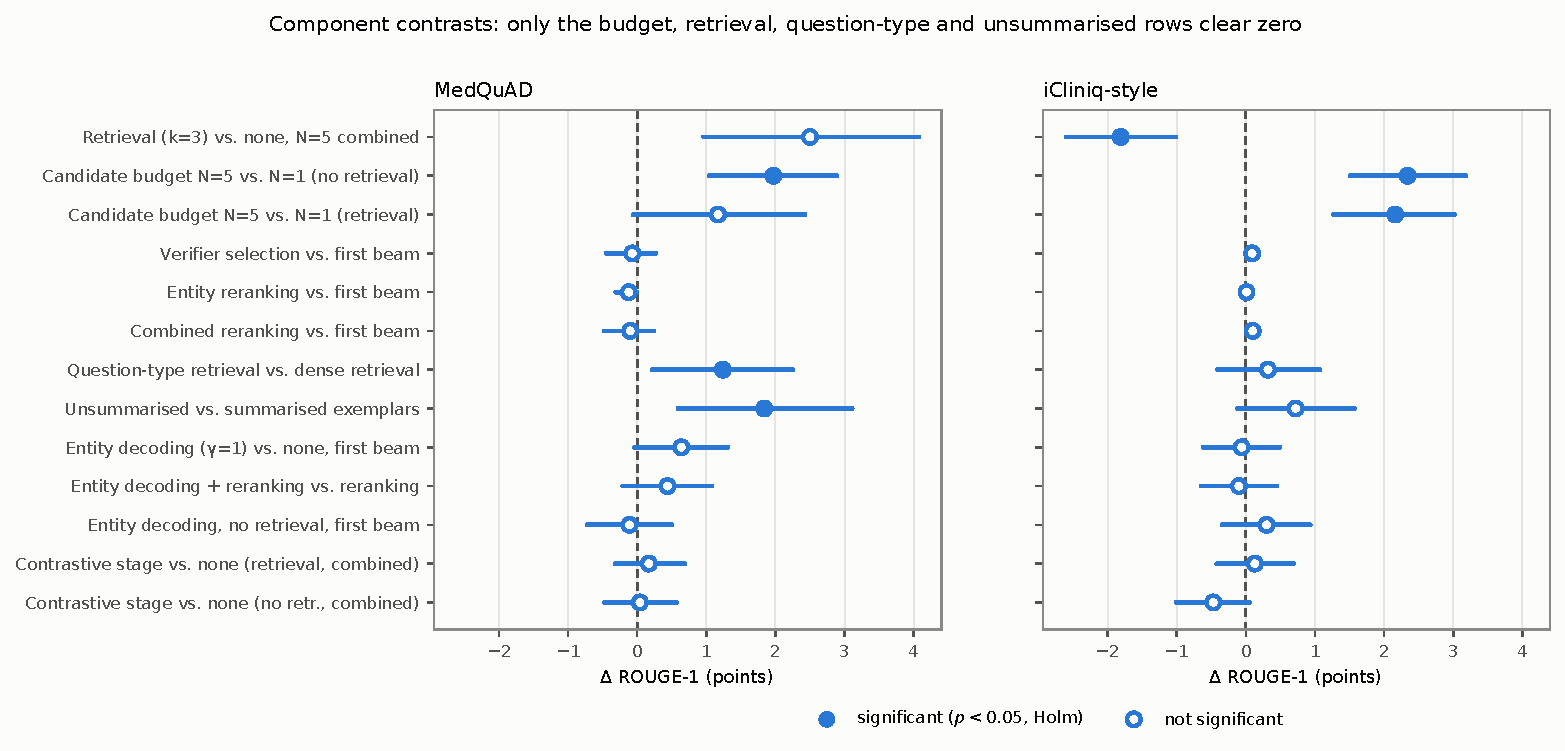
\includegraphics[width=\linewidth]{figures/tab5_primary_components.pdf}
\caption{Component contrasts of Table~\ref{tab:primary-components}, as a forest plot. The figure draws the $\Delta$ROUGE-1 column with its 95\% bootstrap interval; $\Delta$METEOR, $\Delta$BERTScore and the $p$ values for every contrast are in the table, which remains the numeric record.}
\label{fig:tab5-primary-components}
\end{figure*}

\begin{figure*}[!tbp]
\centering
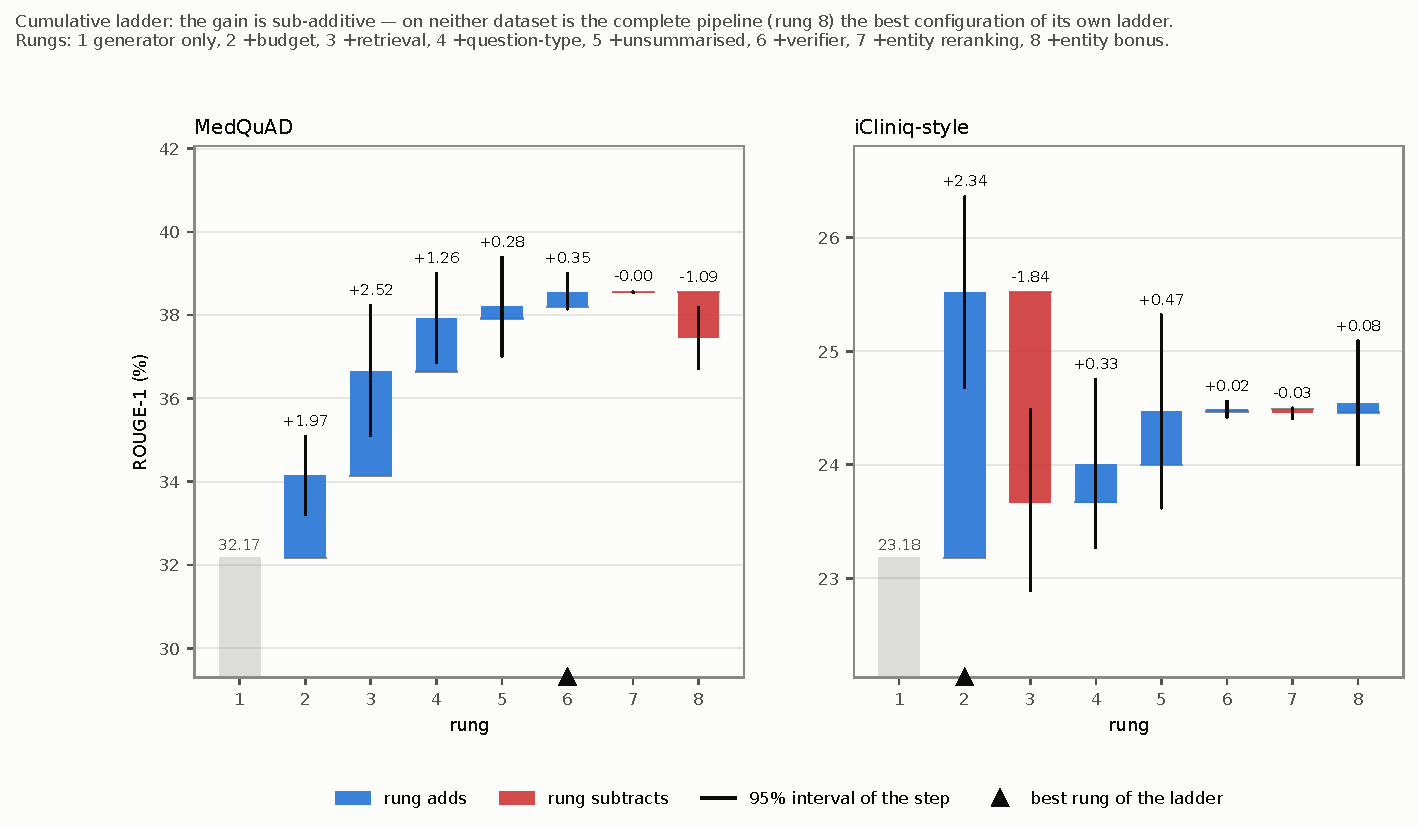
\includegraphics[width=\linewidth]{figures/tab6_7_cumulative_ladder.pdf}
\caption{Cumulative ladder of Tables~\ref{tab:ladder-levels} and \ref{tab:ladder-steps}. The figure draws ROUGE-1 only; ROUGE-2, ROUGE-L, METEOR and BERTScore, each with its own interval, are in the tables. They agree in sign with ROUGE-1 on every rung whose effect exceeds half a point; the rungs where they disagree are all sub-half-point and are reported as no difference.}
\label{fig:tab6-7-cumulative-ladder}
\end{figure*}

\begin{figure*}[!tbp]
\centering
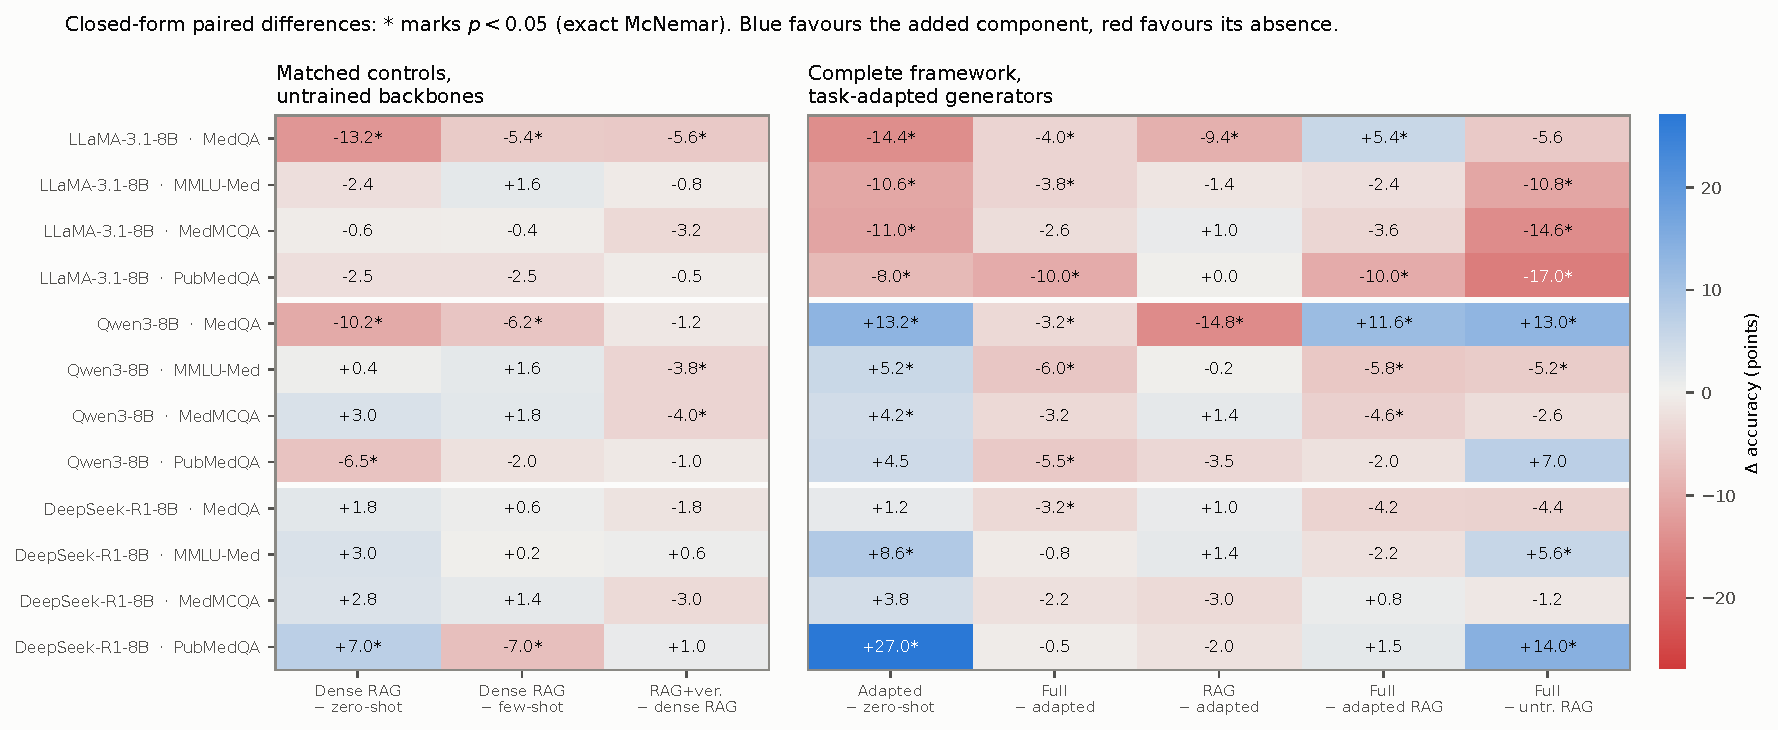
\includegraphics[width=\linewidth]{figures/tab10_13_closedform_paired.pdf}
\caption{Closed-form paired differences of Tables~\ref{tab:cf-matched-paired} and \ref{tab:cf-full-paired}. Cells carry the accuracy difference and mark $p<0.05$; the discordant counts $(a/b)$ and the exact McNemar $p$ for each of the 96 comparisons are in the tables.}
\label{fig:tab10-13-closedform-paired}
\end{figure*}

\begin{figure*}[!tbp]
\centering
\includegraphics[width=\linewidth]{figures/tabD1_D2_gamma_sweep.pdf}
\caption{The $\gamma$ sweep of Tables~\ref{tab:gamma-sweep} and \ref{tab:gamma-retention}. The left panel draws ROUGE-1; the other four quality metrics fall over the same range and are in Table~\ref{tab:gamma-sweep}.}
\label{fig:tabD1-D2-gamma-sweep}
\end{figure*}
